%! TEX root = ../main.tex
\documentclass[main]{subfiles}

\begin{document}
\chapter{開発環境}
\label{cha:environment}
本章では、アプリケーションの開発に使用した環境について説明する。
本研究では、主にフロントエンド開発を中心としたWebアプリケーションの構築を行った。
以下では、使用した言語、ライブラリ、エディタ、バージョン管理システム、実行環境などについて詳述する。
まず、以下に本アプリケーションの開発環境全体を表\ref{tab:dev_environment}に示す。
また図\ref{fig:dev_environment}に、本アプリケーションの開発に関わる要素の関係性を示す。

\begin{table}[htbp]
\centering
\caption{本アプリケーションの開発環境一覧}
\label{tab:dev_environment}
\begin{tabular}{ll}
\hline
項目 & 内容・説明 \\
\hline
開発言語 & JavaScript (ES6以上) \\
フレームワーク & React (v17.0以上) \\
OCRライブラリ & Tesseract.js \\
データ保存 & localStorage \\
バージョン管理 & Git / GitHub \\
エディタ & Visual Studio Code \\
パッケージ管理 & npm \\
実行環境 & Windows 10、Chrome最新版 \\
PCスペック & Intel Core i5、16GB RAM \\
\hline
\end{tabular}
\end{table}

\begin{figure}[htbp]
\centering
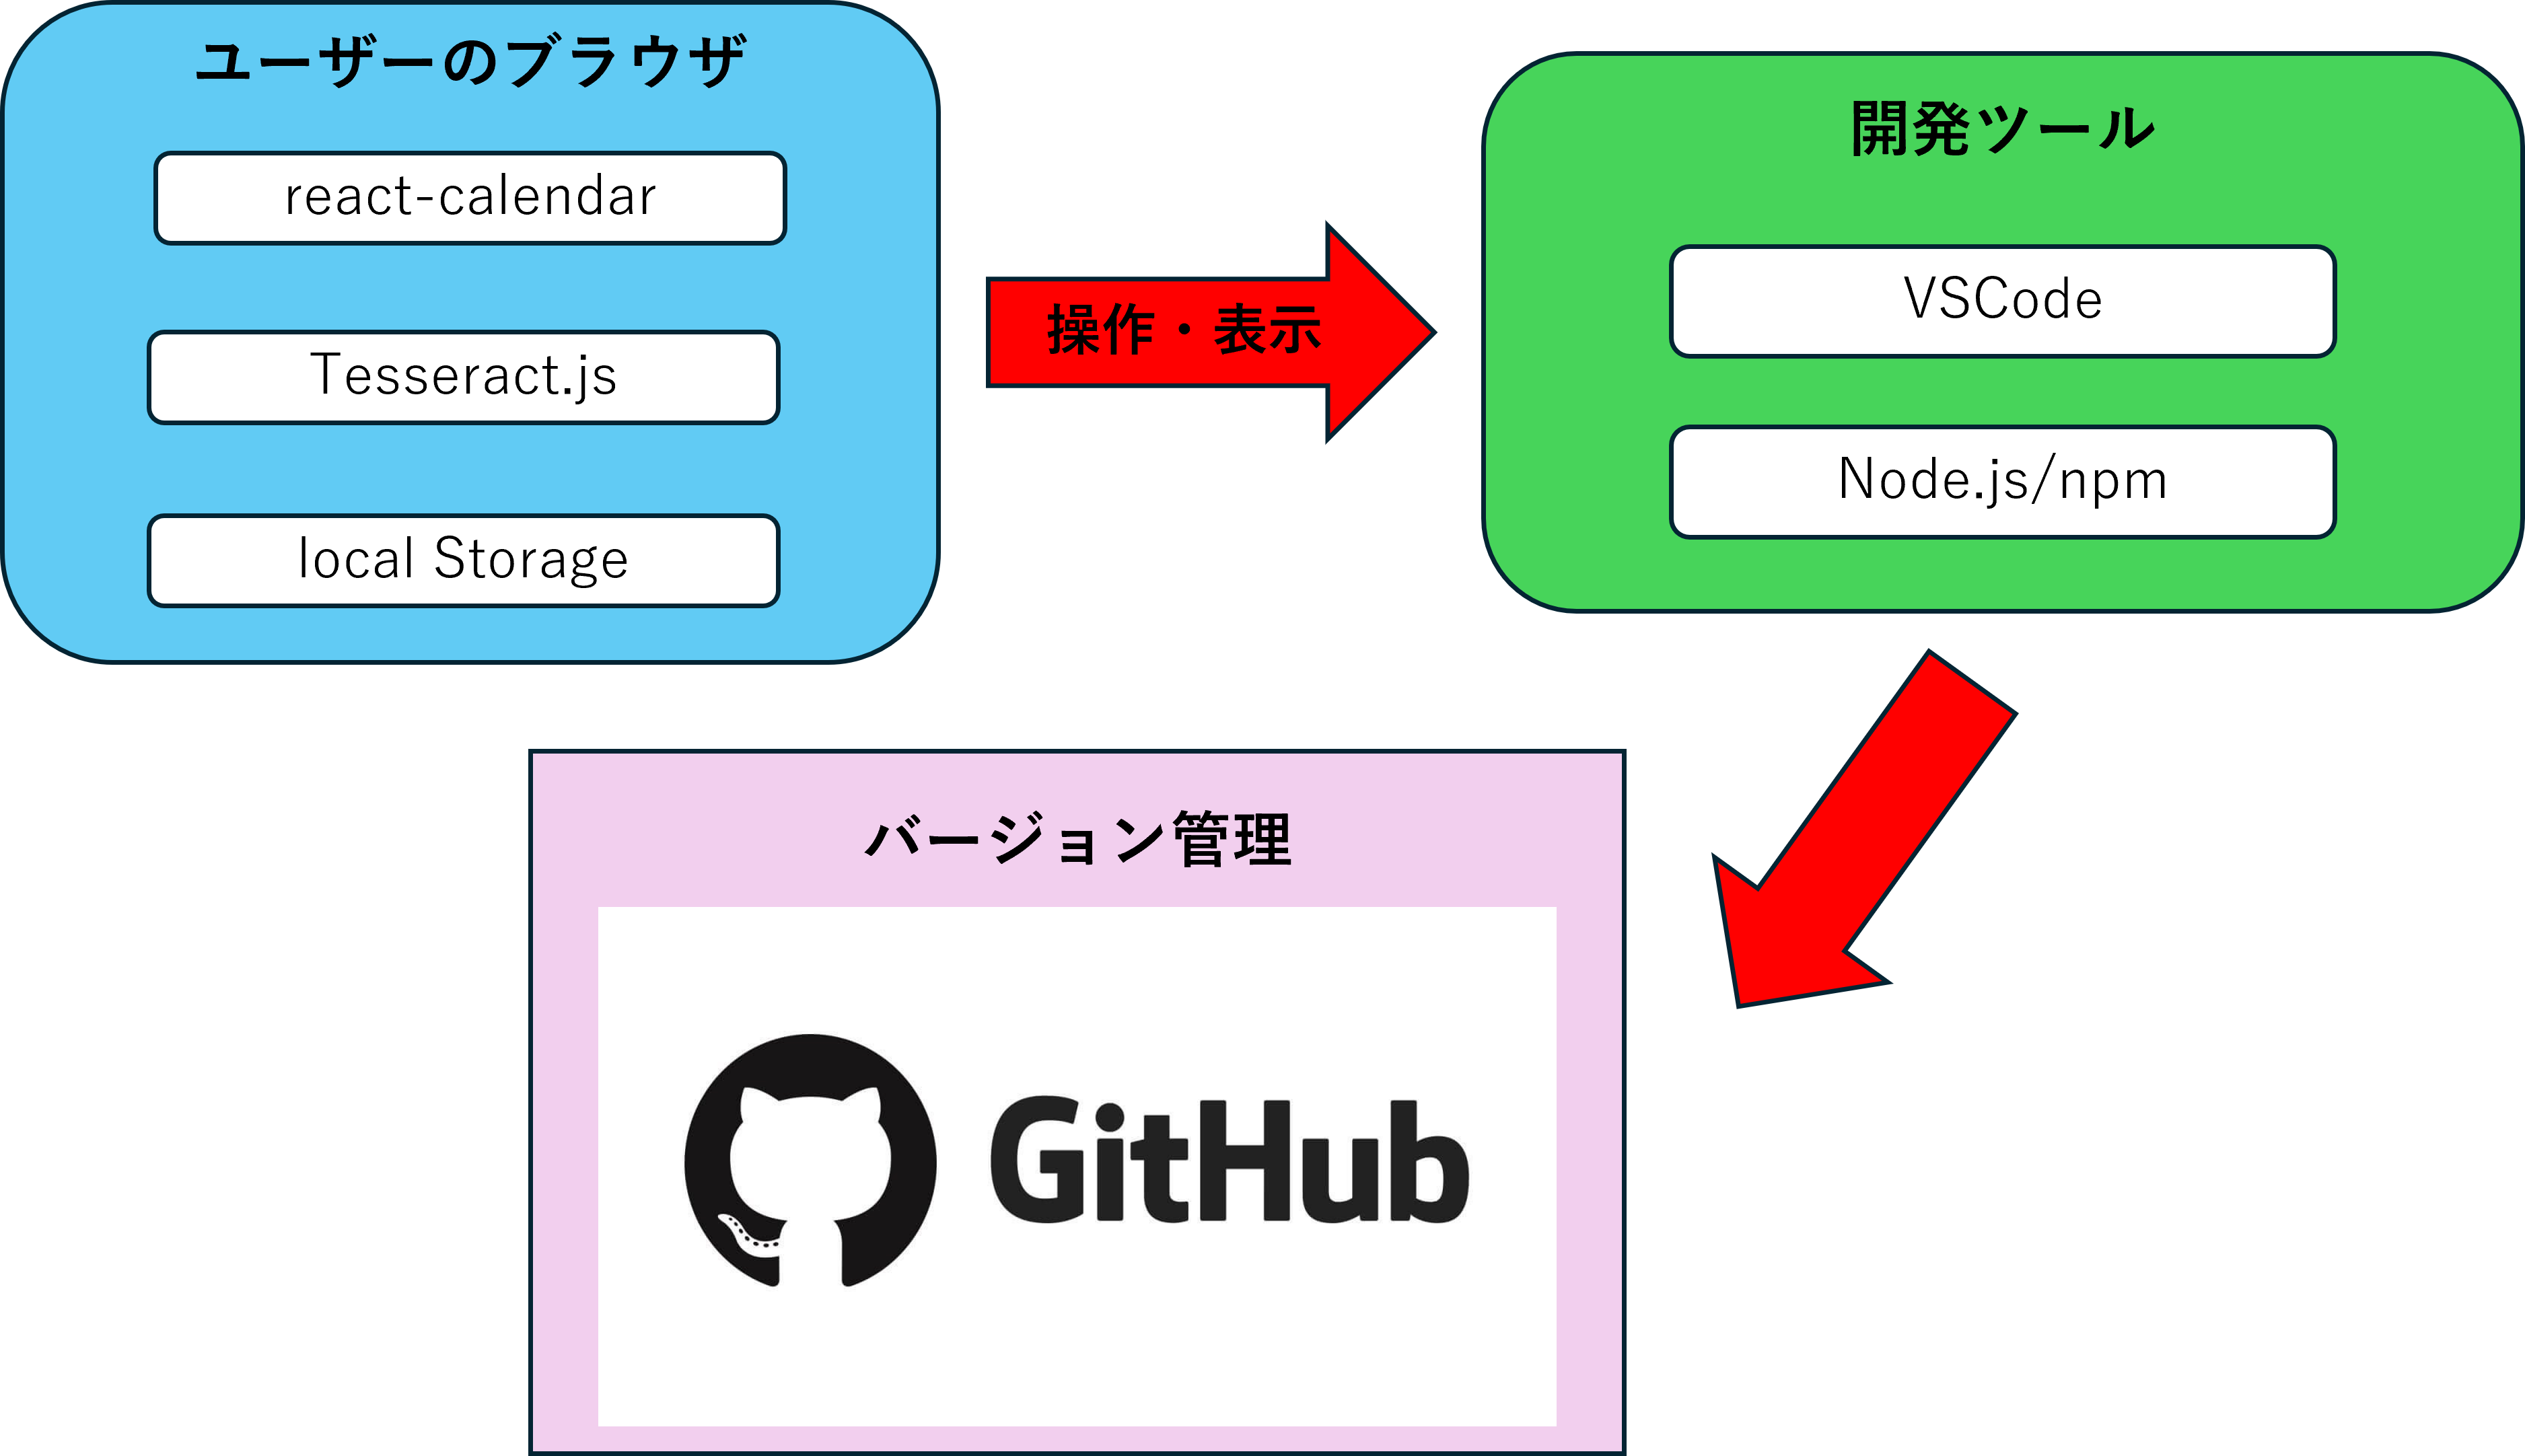
\includegraphics[width=0.9\linewidth]{../figures/environment.png}
\caption{本アプリケーションにおける開発環境の構成図}
\label{fig:dev_environment}
\end{figure}

\section{開発言語とライブラリ}

本アプリケーションでは、主要な開発言語としてJavaScriptを採用した。
JavaScriptはWebブラウザ上で動作し、非同期処理に優れるため、ユーザーとのインタラクションを伴うWebアプリケーションに適している。
UI構築にはReactを導入した。ReactはJavaScriptライブラリであり、コンポーネントベースの設計を可能にする。
仮想DOMによる高速描画や、Hooksを用いた状態管理の簡便さが特長である。
本研究では、特にuseStateおよびuseEffectといった基本的なHooksを活用した。
これにより、ユーザー操作に応じて表示を動的に変化させたり、非同期処理の副作用管理を容易にすることができた。

\begin{table}[htbp]
\centering
\caption{Reactの主要機能とその用途}
\label{tab:react_features}
\begin{tabular}{lp{9cm}}
\hline
\textbf{機能} & \textbf{用途・説明} \\
\hline
useState & コンポーネントの状態管理。ユーザー操作に応じた動的表示に使用。 \\
useEffect & 副作用処理。API呼び出しやDOM操作時に活用。 \\
コンポーネント分割 & UIを部品化し再利用性を向上。保守性の改善にも寄与。 \\
\hline
\end{tabular}
\end{table}

\section{OCRライブラリの利用}

OCR機能には、Tesseract.jsを用いた。Tesseract.jsはGoogleが開発したTesseract OCRエンジンをJavaScriptに移植したライブラリであり、
クライアントサイドで動作する。ユーザーがアップロードしたレシート画像に対して、文字認識処理を実行し、金額や品目、日付などを抽出する。
これにより、サーバーを経由せずに処理が完了するため、プライバシー保護や通信負荷の軽減といった利点がある。
また、Tesseract.jsはWebAssemblyを利用して高速化されており、一般的なブラウザ環境でも実用的な性能をしている。

さらに、Tesseract.jsは学習済みモデルを利用することで、多言語対応が可能である。
日本語対応モデル(jpn.traineddata)を活用することで、国内のレシートに多く見られる縦書きや特殊文字の認識にも対応できる。
また、文字列の前処理には正規表現を用い、余分な空白やノイズ文字の除去を行うことで、抽出精度が向上する。
これらの工夫により、Tesseract.jsの標準機能を最大限に活用しながら、ローカル環境においてより高精度なOCR処理になるように工夫した。

\section{データ保存方式}

本アプリケーションでは、ユーザーの支出データをlocalStorageに保存している。
localStorageはWeb Storage APIの一つで、ユーザーのブラウザに永続的なデータを保存できる機能である。
この方式により、サーバーレスでのデータ保持が可能となり、ユーザーがページを再読み込みした場合でもデータが保持される。
さらに、手動入力した情報やOCRの認識結果もlocalStorageに反映されるよう設計している。
ただし、localStorageは端末やブラウザごとに独立しており、別の環境ではデータが共有されないという制約がある。

この制約に対応する方法として、将来的にはIndexedDBやクラウドストレージとの連携も検討の余地がある。
IndexedDBは構造化データの保存に適しており、大量データや複雑な検索処理に対応できる。
一方、クラウドサービスを用いた同期機能はマルチデバイス間でのデータ共有を実現できるが、実装やセキュリティへの配慮が必要である。

\section{エディタと支援機能}

開発エディタにはVisual Studio Code(以下、VS Code)を用いた。
VS Codeは軽量で高速なコードエディタであり、JavaScriptやReact向けの拡張機能が豊富に提供されている。
Gitとの連携機能により、コードの変更履歴の管理やブランチ操作を行うことができる。
また、構文補完やデバッグ機能、Lintツールとの統合により、コード品質の維持と修正作業をやりやすくなる。
これらの機能を組み合わせて活用することで、日々の開発作業における作業効率とコード保守性を向上させることができた。

\section{開発の進行とツール活用}

開発工程は、要件定義、設計、実装、検証という一般的なプロセスに基づいて進めた。各段階で使用したツールと目的を以下にまとめる。

\begin{table}[htbp]
\centering
\caption{開発段階と使用ツールの対応}
\label{tab:dev_phases}
\begin{tabular}{lll}
\hline
開発段階 & 使用ツール & 目的 \\
\hline
要件定義・設計 & 手書き図、Google Docs & 機能仕様・UI設計 \\
実装 & VS Code、React、npm & コンポーネント開発 \\
検証・分析 & Chrome DevTools、Tesseract.js & OCR精度・UI挙動確認 \\
\hline
\end{tabular}
\end{table}

作業手順を厳密に定義することで、個人開発であっても作業の迷走を防ぎ、効率的に開発を進めることができた。
特にUI構築とOCR処理の統合部分は繰り返しの試行錯誤を伴うため、段階的な実装と小規模なテストを重ねることで安定した動作を実現した。
また、Chrome開発者ツールのプロファイラ機能を用いたパフォーマンスの可視化も有効であった。

\section{実行環境}

アプリケーションは、Windows 10を搭載したPC(Intel Core i5、16GB RAM)上で開発および動作検証を行った。
使用ブラウザは主にChrome最新版であり、動作確認やデバッグにはChrome開発者ツールを利用した。
ブラウザ上で完結する設計としたことで、OS依存の問題も回避した。

検証段階では、異なる解像度のディスプレイやフォントサイズの設定を変えて動作確認を行い、表示崩れや可読性の問題が生じないことを確認した。
また、アプリケーションの軽量性を保つために、画像ファイルの圧縮や不要なアセットの削除も実施し、読み込み時間の短縮に努めた。
このように、限られた環境下でも快適に動作するアプリケーションとなるよう最適化を図った。
実行環境のスペックをまとめた表を以下に示す。

\begin{table}[htbp]
\centering
\caption{実行環境のスペック一覧}
\label{tab:execution_environment}
\begin{tabular}{ll}
\hline
項目 & 内容 \\
\hline
OS & Windows 10 \\
CPU & Intel Core i5 \\
メモリ & 16GB RAM \\
ブラウザ & Google Chrome 最新版 \\
デバッグツール & Chrome 開発者ツール \\
\hline
\end{tabular}
\end{table}


\end{document}